\chapter[Desenvolvimento]{Desenvolvimento} \label{cap:desenvolvimento}
    O trabalho de muitos desenvolvedores de arquiteturas de alocação de tarefa para sistemas de vários robôs pode passar desapercebido ou ser ignorado por pessoas que buscam resolver esse problema. A falta de uma documentação mínima leva a maioria dos seus usuários a desistir de compreender tais trabalhos. Além disso, a configuração dessas arquiteturas pode deixar seus usuários confusos devido a imensidão de parâmetros existentes. Levando esses fatos em consideração, foi desenvolvido o pacote \textit{rqt\_mrta} que implementa uma aplicação gráfica para o auxílio na utilização de arquiteturas MRTA do ROS.
        
    Este capítulo apresenta detalhes pertinentes sobre o desenvolvimento dos pacotes \textit{rqt\_mrta} para o \textit{framework} ROS.
    
    \lstset{
        language=XML,
        breaklines=true,
        frameround=ffff,
        frame=single,
        rulecolor=\color{black},
        autogobble=true,
        morekeywords={
            xml, encoding,
            package, format,
            name,
            version,
            description,
            maintainer, email,
            author,
            license,
            url, type,
            buildtool_depend,
            build_depend,
            run_depend,
            export,
                metapackage,
                plugin,
                rqt_gui,
                alliance,
                rqt_mrta, application, architecture,
        xml, version, encoding,
            rqt_mrta, format,
                architecture,
                    name,
                    robots,
                        busy_robots,
                        idle_robots,
                        config_id,
                        launch_id,
                        robot_0,
                        robot_1,
                    tasks,
                        incoming_tasks,
                        task_0,
                        task_1,
                    allocations,
                        allocated_tasks,
                        type,
                        topic,
                            name,
                            type,
                            field,
                            timeout,
                            tool_tip,
                configs,
                    config_0,
                        id,
                        value,
                        param_0,
                        param_1,
                        params_0,
                        params_1,
                        params_2,
                        params_3,
                        params_4,
                        params_5,
                        params_6,
                        array_0,
                        array_1,
                            tool_tip,
                launches,
                    launch_0,
                    launch_1,
                    includes,
                        include_0,
                        include_1,
                            file,
                            args,
                                arg_0,
                                arg_1,
                widgets,
                    widget_0,
                        plugin_name,
        }
    }
    
    O pacote desenvolvido atende dois tipos de usuários: desenvolvedores de arquiteturas MRTA e usuários de arquiteturas MRTA. Desenvolvedores de arquiteturas MRTA podem utilizar este \textit{software} para o registro e definição da arquitetura desenvolvida. Ao fazê-los, sua arquitetura estará disponível para o uso de usuários de arquitetura MRTA através do \textit{rqt\_mrta}. Por sua vez, os usuários de arquitetura MRTA podem utilizar o \textit{rqt\_mrta} para a definição do seu problema MRTA, para escolher uma arquitetura disponível para uso e também para a configuração da arquitetura escolhida conforme a definição do seu problema. Ao final desse procedimento, a aplicação salva os arquivos necessários para o uso da arquitetura escolhida em um novo pacote ROS.
    
    Para isso, existem dois arquivos de configuração, um para a configuração da arquitetura e outro para a configuração do problema. Ambos arquivos possuem a extensão XML (Extensible Markup Language). Ao serem carregados pela aplicação, esta se adapta para tratar o problema MRTA definido, utilizando a arquitetura escolhida. 
    
    Esse pacote está em conformidade com a convenção\footnote{\url{http://wiki.ros.org/ROS/Patterns/Conventions}} de nomes de pacote do ROS. O nome de pacotes que proveem ferramentas GUI baseada em Qt para o ROS deve ter o prefixo ``\textit{rqt\_}''. Esta interface gráfica utiliza a API em C++ do \textit{framework rqt} e pode ser utilizada como uma aplicação \textit{standalone}\footnote{Tipo de programa que não precisa de \textit{software} auxiliar para a sua execução.} ou, então, como um \textit{plugin} que pode ser acoplado em uma janela do \textit{rqt\_gui}\footnote{\url{http://wiki.ros.org/rqt_gui}} juntamente com outras ferramentas gráficas (vide Seção \ref{subsec:ros_gui}) do ROS.
    
    Este projeto foi concebido utilizando o padrão arquitetural MVC (\textit{Model-View-Controller}), sendo assim dividido em três camadas: dados (\textit{model}), apresentação (\textit{view}) e regra de negócio (\textit{controller}).
    
    A seguir serão detalhados os arquivos de configuração de arquitetura e aplicação, bem como, as camadas do modelo, de visualização e controle.
        
    \section{Arquivo de configuração de arquitetura} \label{sec:arch_config}
        O arquivo de configuração de arquitetura tem como propósito:
        
        \begin{itemize}
            \item classificar a arquitetura segundo a taxonomia sugerida por \citeonline{ref:gerkey2004taxonomy};
            \item identificar os parâmetros necessários para sua configuração inicial;
            \item identificar os arquivos necessários para a sua inicialização;
            \item associar os arquivos de parâmetros com os arquivos de inicialização;
            \item identificar as ferramentas gráficas para a análise do desempenho da arquitetura em tempo de execução.
        \end{itemize}
        
        \subsection{Formatação} \label{subsec:arch_config_fmt}
            Esse arquivo de extensão XML conta com quatro \textit{tags} principais: \textit{architecture}, \textit{configs}, \textit{launches} e \textit{widgets}. A seguir, é mostrada uma simplificação de um arquivo de configuração de arquitetura. No entanto, o Apêndice \ref{app:arch_config} apresenta um exemplo completo, contendo as configurações da arquitetura implementada no pacote ROS \textit{alliance}, o qual será discutido na Seção \ref{cap:resultados}.
            
            \begin{lstlisting}
                <rqt_mrta>
                  <architecture>
                    <name>ALLIANCE</name>
                    <robots>
                      <type>ST</type>
                      <busy_robots>
                        <topic>
                          ...
                        </topic>
                      </busy_robots>
                      <config_id>alliance_params</config_id>
                      <idle_robots>
                        <topic>
                          ...
                        </topic>
                      </idle_robots>
                      <launch_id>alliance</launch_id>
                    </robots>
                    <tasks>
                      <type>SR</type>
                      <incoming_tasks>
                        <topic>
                          ...
                        </topic>
                      </incoming_tasks>
                    </tasks>
                    <allocations>
                      <type>IA</type>
                      <allocated_tasks>
                        <topic>
                          ...
                        </topic>
                      </allocated_tasks>
                    </allocations>
                  </architecture>
                  <configs>
                    <config_0>
                      <id>alliance_params</id>
                      ...
                    <config_0>
                    ...
                  </configs>
                  <launches>
                    <launch_0>
                      <id>alliance</id>
                      ...
                    </launch_0>
                    ...
                  </launches>
                  <widgets>
                    <widget_0>
                      <plugin_name></plugin_name>
                    </widget_0>
                    ...
                  </widgets>
                </rqt_mrta>
            \end{lstlisting}
            
            A \textit{tag architecture} possui as \textit{tags name}, \textit{robots}, \textit{tasks} e \textit{allocations}, as quais contêm, respectivamente, informações sobre o nome da arquitetura e considerações sobre os robôs, tarefas e alocações do problema MRTA. A \textit{tag robots} agrupa informações sobre o tipo dos robôs do problema MRTA que ela resolve e, através da \textit{tag topic}, dá detalhes pertinentes para a verificação da alteração de estado dos robôs. A \textit{tag topic} será explicada a seguir. A \textit{tag tasks}, por sua vez, traz dados sobre o tipo de tarefa que a arquitetura considera, bem como, informações para a identificação de novas tarefas que surgem no sistema. A \textit{tag allocations} classifica o tipo de alocação tratada pela arquitetura, assim como, traz informações para a verificação de alteração de estado da alocação. Essas informações são úteis para ajudar o usuário a escolher uma arquitetura válida para o seu problema MRTA. Além disso, elas permitirão a identificação dos estados dos robôs, tarefas e alocações em tempo de execução.
            
            \begin{lstlisting}
                <topic>
                  <name>/allocations</name>
                  <type>mrta_msgs/Allocation</type>
                  <field>header/frame_id</field>
                  <timeout>2.5</timeout>
                </topic>
            \end{lstlisting}
            
            As \textit{tags busy\_robots}, \textit{idle\_robots}, \textit{incoming\_tasks} e \textit{allocated\_tasks} têm a \textit{tag topic} dentro do seu escopo. Esta \textit{tag}, por sua vez, possui quatro \textit{tags}: \textit{name}, \textit{type}, \textit{field} e \textit{timeout}. Elas informam o nome do tópico, o tipo da mensagem transportada pelo tópico, o campo da mensagem e o tempo máximo considerado sem receber uma nova mensagem. Através dessas informações, a aplicação é capaz de identificar o estado dos robôs, tarefas e alocações do sistema.
            
            A \textit{tag configs} reúne um grupo de \textit{templates} para a geração de arquivos de parâmetros que serão utilizados na inicialização dos nós da arquitetura. Esses arquivos de parâmetros possuem extensão YAML (\textit{YAML Ain't Markup Language}). Cada \textit{template} é definida dentro de uma \textit{tag config}, a qual possui um identificador que pode ser associado a um robô. Nessa situação, será pedido ao usuário durante a criação de um novo problema o preenchimento dos parâmetros para cada robô do sistema. Aqueles que não são associados aos robôs necessitam ser preenchidos apenas uma vez. As seguintes \textit{tags} são utilizadas para a criação de uma \textit{template}:
            
            %Para criar um \textit{template} de um arquivo de parâmetros basicamente se faz uso de três \textit{tags}: \textit{params}, \textit{array} e \textit{param}. As duas primeiras são coleções de parâmetros, a única diferença entre elas é que \textit{array} define uma coleção de parâmetros que se repete um dado número de vezes. A \textit{tag param} define o nome, o valor, o tipo, a instrução e o valor padrão de um parâmetro. 
            %
            \begin{itemize}
                \item \textit{id}: identifica o arquivo de parâmetros, seu valor pode ser usado para associar essa \textit{template} com os robôs;
                \item \textit{param}: traz informações importantes sobre o preenchimento de dados de um parâmetro. Esta \textit{tag} contem as \textit{tags name}, \textit{type}, \textit{value}, \textit{default} e \textit{tool\_tip}. Quando a \textit{tag default} não é dada, o parâmetro em questão é considerado obrigatório;
                \item \textit{params}: armazena uma coleção de parâmetros, seus filhos podem ser \textit{tags} do tipo \textit{param}, \textit{params} e \textit{array};
                \item \textit{array}: armazena uma coleção de parâmetros, seus filhos podem ser \textit{tags} do tipo \textit{param}, \textit{params} e \textit{array}; além disso, deve ser filha de uma \textit{tag params} e ter uma \textit{tag param} irmã cujo valor da \textit{tag name} deve ser \textit{size}. Através deste parâmetro, é possível identificar o número de vezes que a coleção de parâmetros armazenados pela \textit{tag array} irá se repetir;
                \item \textit{name}: informa o nome do parâmetro;
                \item \textit{type}: informa o tipo do valor do parâmetro, assim seus valores podem ser \textit{bool}, \textit{int}, \textit{double} ou \textit{string};
                \item \textit{value}: armazena o valor do parâmetro;
                \item \textit{tool\_tip}: traz uma instrução para contextualizar o usuário durante o preenchimento do parâmetro.
            \end{itemize}
            %
            A seguir é mostrado um trecho da \textit{tag configs} extraído do Apêndice \ref{app:arch_config}.
            
            \begin{lstlisting}
              <configs>
                <config_0>
                  <id>alliance_params</id>
                  <param_0>
                    <name>name</name>
                    <type>string</type>
                    <tool_tip>Enter the robot name.</tool_tip>
                  </param_0>
                  ...
                  <params_6>
                    <name>behaviour_sets</name>
                    <param_0>
                      <name>size</name>
                      <type>int</type>
                      <value>@array_size@</value>
                      <tool_tip>Enter the number of behaviour sets that the robot have.</tool_tip>
                    </param_0>
                    <array_1>
                      <name>behaviour_set@index@</name>
                      <param_0>
                        <name>task_id</name>
                        <type>string</type>
                        <tool_tip>Enter the task id in which this behaviour set is related to.</tool_tip>
                      </param_0>
                      ...
                    </array_1>
                  </params_6>
                  ...
                </config_0>
                ...
              </configs>
            \end{lstlisting}
            
            A \textit{tag launches} é uma coleção de \textit{templates} para a geração de arquivos de inicialização de nós do ROS. A extensão desses arquivos é do tipo LAUNCH, os quais podem ser utilizados pela ferramenta \textit{roslaunch}\footnote{http://wiki.ros.org/roslaunch} para a inicialização do sistema no ROS. Cada \textit{template} de arquivo de inicialização é definida por uma \textit{tag launch}. Para incluir um arquivo de inicialização dentro da \textit{template} deve-se utilizar uma \textit{tag include}, indicando seus argumentos através da \textit{tag arg} e a localização do arquivo desejado. As demais \textit{tags} de um arquivo de inicialização do ROS não são suportadas, pois todos os demais recursos podem ser utilizados dentro do arquivo incluído pela \textit{template}. A seguir é mostrado um trecho da \textit{tag launches} extraído do Apêndice \ref{app:arch_config}.
            
            \begin{lstlisting}
              <launches>
                <launch_0>
                  <id>alliance</id>
                  <includes>
                    <include_0>
                      <file>$(find alliance)/launch/alliance.launch</file>
                      <args>
                        <arg_0>
                          <name>robot_id</name>
                          <value>@robot_id@</value>
                        </arg_0>
                        <arg_1>
                          <name>robot_params</name>
                          <value>$(find @package@)/launch/@robot_id@_alliance_params.yaml</value>
                        </arg_1>
                        ...
                      </args>
                    </include_0>
                    ...
                  </includes>
                </launch_0>
                ...
              </launches>
            \end{lstlisting}
            
            Finalmente, pode ser informado ao \textit{plugin} uma coleção de outros \textit{plugin} desenvolvidos para a análise da arquitetura em tempo de execução. Para isso, deve-se usar a \textit{tag widgets} informando o nome de cada \textit{plugin}.
        
        \subsection{Registro da arquitetura} \label{subsec:arch_config_rgst}
            No entanto, torna-se necessário um mecanismo de busca capaz de identificar pacotes ROS que contenham arquivos de configuração de arquitetura; pois, assim, será possível auxiliar o usuário final a escolher uma arquitetura que resolva o seu problema MRTA.
            
            A biblioteca \textit{rospack}\footnote{\url{http://wiki.ros.org/rospack}} possui diversas ferramentas de busca de informação de pacotes existentes no sistema de arquivos do ROS. Dentre elas, a ferramenta \textit{rospack plugin} examina os pacotes ROS procurando por aqueles que dependem diretamente do pacote dado, extraindo de cada um deles seu nome acompanhado pelo valor do atributo requisitado. Logo, é possível utilizar esse mecanismo em benefício deste projeto ao adicionar uma dependência do \textit{rqt\_mrta} ao pacote da arquitetura, assim como, exportar a localização relativa do seu arquivo de configuração. 
            
            Portanto, para que o \textit{rqt\_mrta} tenha visibilidade das arquiteturas configuradas, são necessárias algumas alterações no arquivo manifesto do pacote que implementa cada uma delas. Primeiramente, é necessário adicionar a dependência em tempo de execução do pacote \textit{rqt\_mrta}. Para isso, é necessário adicionar ao arquivo \textit{package.xml} do pacote desejado a seguinte linha:
            
            \begin{lstlisting}
                <run_depend>rqt_mrta</run_depend>
            \end{lstlisting}
            
            A segunda alteração necessária exportará a localização do arquivo de configuração dentro do pacote em questão. Para isso, deve-se adicionar a seguinte linha dentro do escopo da \textit{tag export} do arquivo \textit{package.xml}:
            
            \begin{lstlisting}
                <rqt_mrta architecture="${prefix}/rqt_mrta.xml"/>
            \end{lstlisting}
            
            Note que, neste caso, deve ser requisitado o atributo \textit{architecture}. Será visto adiante que este atributo tem outro nome quando se trata de arquivos de configuração de aplicação.
            
            Dessa forma, o arquivo manifesto do pacote (\textit{package.xml}) deve conter, obrigatoriamente, as linhas abaixo. Deve-se respeitar a hierarquia das \textit{tags}.
            
            \begin{lstlisting}
                <package>
                  ...
                  <run_depend>rqt_mrta</run_depend>
                  ...
                  <export>
                    ...
                    <rqt_mrta architecture="${prefix}/plugin.xml"/>
                    ...
                  </export>
                  ...
                </package>
            \end{lstlisting}
            
            O Apêndice \ref{app:arch_manifest} mostra um exemplo de arquivo manifesto de um pacote configurado para ser uma arquitetura MRTA do ponto de vista do \textit{rqt\_mrta}. Note a dependência em tempo de execução do pacote \textit{rqt\_mrta}, bem como, a exportação da sua \textit{tag} com o atributo \textit{architecture}.
    
    \section{Arquivo de configuração de aplicação} \label{sec:app_config}
        Um arquivo de configuração de aplicação informações gerais da aplicação, identifica os robôs do sistema e armazena as escolhas feitas pelo usuários durante a parametrização da arquitetura. Será apresentado o formato deste arquivo e também como este arquivo é reconhecido pelo \textit{rqt\_mrta}.
        
        \subsection{Formatação} \label{subsec:app_config_fmt}
            Esse arquivo de extensão XML conta com três \textit{tags} principais: \textit{application} e \textit{configs}, \textit{launches}. A seguir, é mostrada uma simplificação de um arquivo de configuração de aplicação. No entanto, o Apêndice \ref{app:app_config} apresenta um exemplo completo, contendo as configurações da aplicação \textit{patrulha}, a qual é discutida na Seção \ref{cap:resultados}.
            
            \begin{lstlisting}
              <rqt_mrta>
                <application>
                  <architecture>alliance</architecture>
                  <name>Patrulha na UNIFEI</name>
                  <robots>
                    <robot_0>
                      <id>/robot1</id>
                      <tasks>
                        <task_0>
                          <id>wander</id>
                        </task_0>
                        ...
                      </tasks>
                    </robot_0>
                    ...
                  </robots>
                </application>
                <configs>
                  ...
                </configs>
                <launches>
                  ...
                </launches>
              </rqt_mrta>
            \end{lstlisting}
        
            A \textit{tag application} armazena metadados sobre o problema MRTA e composta pelas seguintes \textit{tags}:
            
            \begin{itemize}
                \item \textit{architecture}: armazena o nome do pacote que implementa a arquitetura escolhida;
                \item \textit{name}: armazena o nome da aplicação;
                \item \textit{robots}: agrupa uma coleção de \textit{tags} do tipo \textit{robot};
                \item \textit{robot}: possui uma \textit{tag id} e uma tag \textit{tasks};
                \item \textit{tasks}: reune um conjunto de \textit{tags} do tipo \textit{task};
                \item \textit{task}: possui uma \textit{tag id};
                \item \textit{id}: identifica robôs e tarefas no sistema.
            \end{itemize}
            
            As seguintes \textit{tags} estão agrupadas na \textit{tag application}
            A \textit{tag application} agrupa metadados sobre o problema, como o nome da aplicação e o nome do pacote que implementa a arquitetura MRTA escolhida. Além disso, a \textit{tag robots} identifica os robôs do sistema. Este arquivo também armazena os parâmetros adotados durante a criação do problema MRTA. Isso permite que os seus valores possam ser atualizados. Por fim, este arquivo também guarda a estrutura dos arquivos de inicialização do ROS que foram gerados após sua criação. 
        
            As \textit{tags configs} e \textit{launches} permitem a reconfiguração da arquitetura e da aplicação após sua geração. Elas possuem a mesma estrutura descrita em \ref{subsec:arch_config}. Porém, este arquivo não possui \textit{tags} do tipo \textit{array}, pois cada uma delas foi substituída por uma coleção de \textit{tags} do tipo \textit{params}, conforme o exemplo extraído do Apêndice \ref{app:app_config} que se seute.
            
            \begin{lstlisting}
              <configs>
                <config_0>
                  ...
                  <params_5>
                    <name>sensors</name>
                    <param_0>
                      <default></default>
                      <name>size</name>
                      <tool_tip>Enter the number of sensors that the robot have.</tool_tip>
                      <type>int</type>
                      <value>2</value>
                    </param_0>
                    <params_1>
                      <name>sensor0</name>
                      <param_0>
                        <default></default>
                        <name>plugin_name</name>
                        <tool_tip>Enter the sensor plugin name.</tool_tip>
                        <type>string</type>
                        <value>alliance_test/odometry</value>
                      </param_0>
                      ...
                    </params_1>
                    <params_2>
                      <name>sensor1</name>
                      <param_0>
                        ...
                      </param_0>
                      ...
                    </params_2>
                  </params_5>
                  ...
                </config_0>
                ...
              </configs>
            \end{lstlisting}
            
        \subsection{Registro da aplicação} \label{subsec:app_config_rgst}
            Semelhante às configurações de arquitetura, é desejável que o \textit{plugin rqt\_mrta} tenha visibilidade dos pacotes que contêm os dados e as configurações de um problema MRTA. Novamente, são necessárias algumas alterações no arquivo \textit{package.xml} do pacote desejado, semelhante àquelas realizadas para um pacote que implementa uma arquitetura MRTA. Entretanto, a única diferença está no nome do atributo da \textit{tag} de exportação do \textit{rqt\_mrta}, a qual passa a ser \textit{application} ao invés de \textit{architecture}, conforme visto abaixo.
            
            \begin{lstlisting}
                <package>
                  ...
                  <run_depend>rqt_mrta</run_depend>
                  ...
                  <export>
                    ...
                    <rqt_mrta application="${prefix}/plugin.xml"/>
                    ...
                  </export>
                  ...
                </package>
            \end{lstlisting}
            
            O Apêndice \ref{app:app_manifest} mostra um exemplo de arquivo manifesto de um pacote configurado para ser um problema MRTA do ponto de vista do \textit{rqt\_mrta}. Note a dependência em tempo de execução do pacote \textit{rqt\_mrta}, bem como, a exportação da sua \textit{tag} com o atributo \textit{application}.
    
    \section{Camada do modelo} \label{subset:rqt_mrta_model}
        A camada de modelo facilita a importação e exportação dos dados dos arquivos de configuração detalhados em \ref{subsec:arch_config} e \ref{subsec:app_config}. Conforme mostra a Figura \ref{fig:rqt_mrta_model_uml}, a relação entre as classes do modelo se apresenta como um grafo, semelhantemente à estrutura dos arquivos de configuração de arquitetura e aplicação. Ao utilizar o padrão de projeto de \textit{software} cadeia de responsabilidade \cite{ref:gamma1993design} nesta organização de classes, simplificou-se a geração dos arquivos de inicialização, de parâmetros, configuração de arquitetura e aplicação, assim como, a leitura desses dois últimos tipos de arquivo.
        
        \begin{figure}[p]
            \centering
            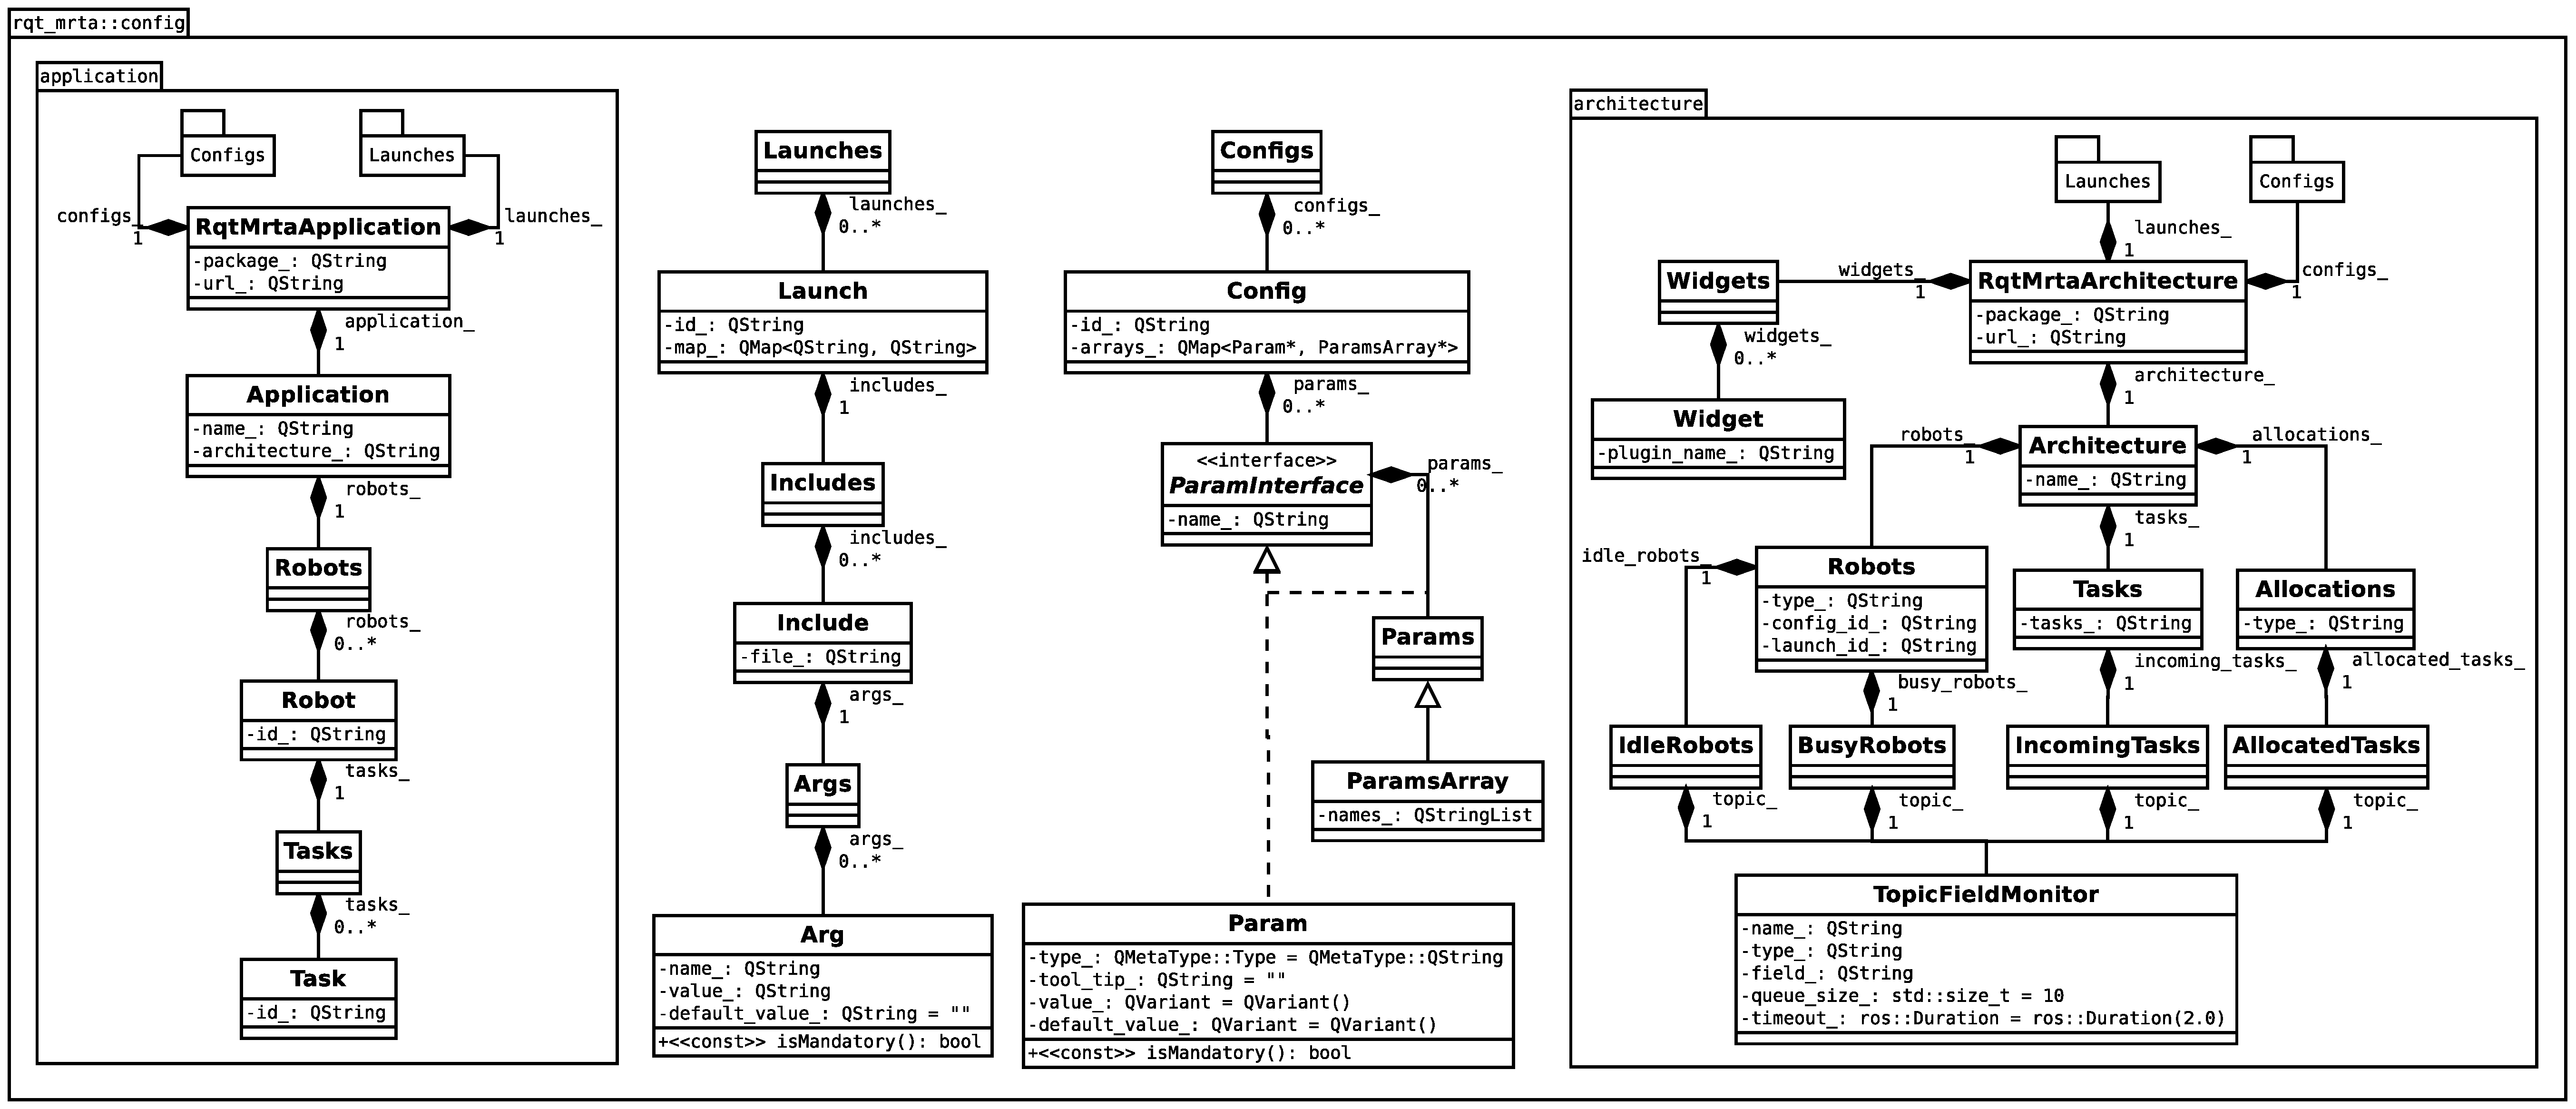
\includegraphics[width=.97\textheight,angle=90]{Figuras/3_desenvolvimento/rqt_mrta_model_uml.eps}
            \caption{Diagrama de classes da camada do modelo.} \label{fig:rqt_mrta_model_uml}
        \end{figure}
        
        Cada classe mostrada na Figura \ref{fig:rqt_mrta_model_uml} representa uma \textit{tag} não folha. E as \textit{tags} folhas são membros de alguma classe do modelo. Alguma dessas classes possuem métodos utilitários que ajudam na geração de arquivos. São elas:
        
        \begin{itemize}
            \item \textit{RqtMrtaArchitecture}:
            \item \textit{RqtMrtaApplication}:
            \item \textit{Launches}:
            \item \textit{Launch}:
            \item \textit{Configs}:
            \item \textit{Config}:
            
        \end{itemize}
        
    \section{Camada de visualização} \label{subsec:rqt_mrta_view}
        O Qt \cite{ref:yafei2012qt} possui uma ferramenta chamada \textit{Qt Designer} que permitiu o desenvolvimento da camada de apresentação (\textit{view}) deste projeto, pois ela representa graficamente a disposição dos componentes Qt para a customização de janelas (\textit{widgets}, \textit{dialogs} e \textit{wizards}). A partir dessas representações foram gerados arquivos de extensão UI (\textit{User Interface}) que armazenam a árvore de relação entre os componentes Qt e formata os dados em XML. Finalmente, em tempo de compilação, os arquivos UI foram convertidos para classes codificadas em C++.
        
        A Figura \ref{fig:example_new_app} mostra as telas do \textit{wizard} para a criação de uma nova aplicação, onde são definidos seus os dados gerais, é selecionado uma das arquiteturas registradas, são definidos os robôs do sistema, bem como, as tarefas que cada um é capaz de realizar. Em seguida, cada arquivo necessário para parametrizar a arquitetura escolhida é preenchido e, finalmente, é mostrado quais arquivos e pastas serão criados a partir das informações dadas. 
        
        Ao final deste procedimento, será criado um pacote contendo o arquivos manifesto (configurado conforme \ref{subsec:app_config_rgst}), CMakeLists.txt e de configuração de aplicação. Em seguida, são gerados os arquivos de parâmetro e de inicialização a partir dos dados inseridos pelo usuário. Os arquivos de parâmetro serão agrupados na pasta \textit{config} do pacote gerado e os arquivos de inicialização serão agrupados na pasta \textit{launch} do pacote gerado.
        
        \begin{figure}[htb]
            \centering
            \subfloat[Dados gerais da aplicação.]{
                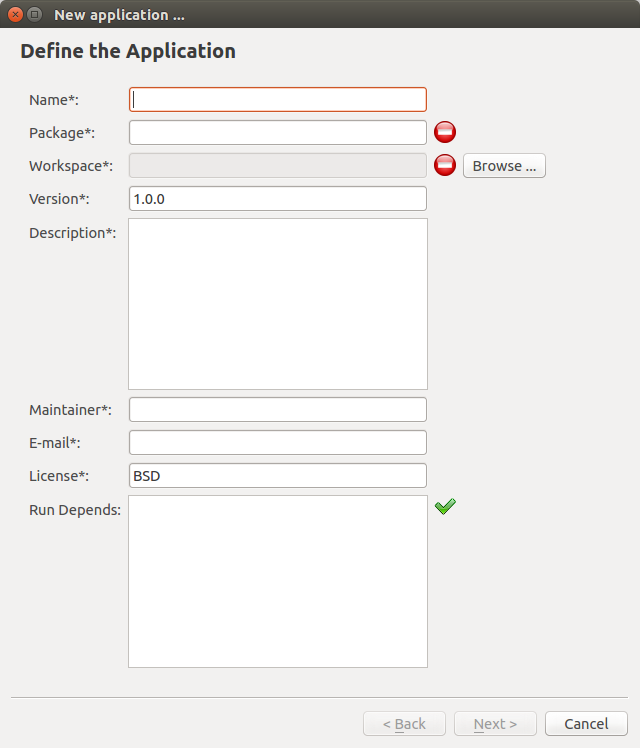
\includegraphics[width=.31\textwidth]{Figuras/3_desenvolvimento/example_def_app.png}
                \label{fig:example_def_app}
            }
            \subfloat[Escolha da arquitetura.]{
                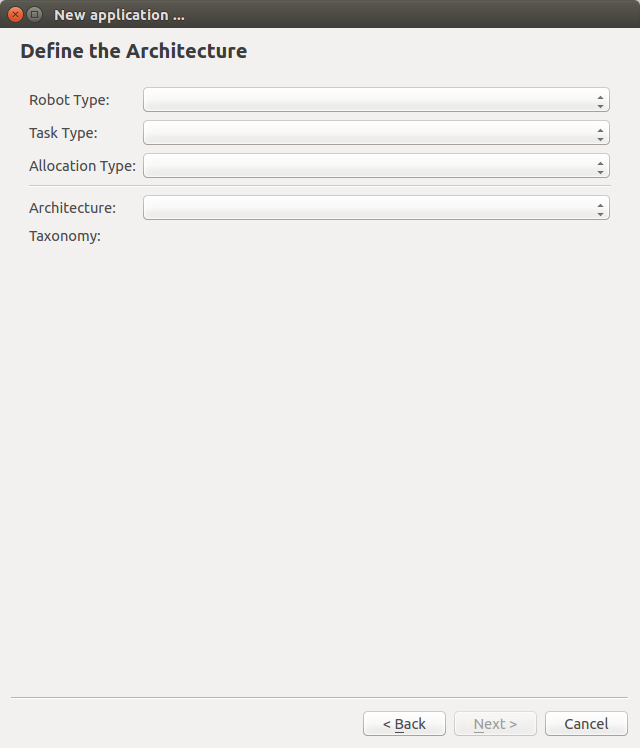
\includegraphics[width=.31\textwidth]{Figuras/3_desenvolvimento/example_def_arch.png}
                \label{fig:example_def_arch}
            }
            \subfloat[Definição dos robôs do sistema.]{
                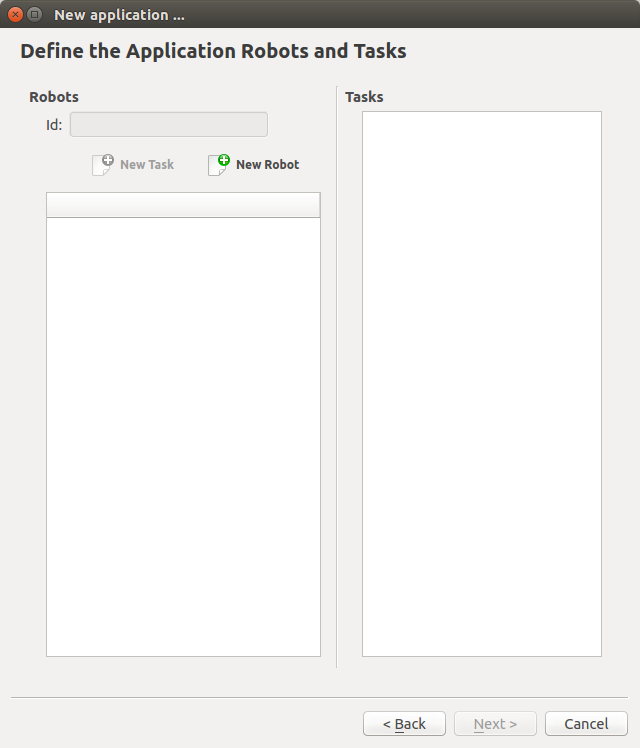
\includegraphics[width=.31\textwidth]{Figuras/3_desenvolvimento/example_def_robots.png}
                \label{fig:example_def_robots}
            }
            
            \subfloat[Parametrização da arquitetura.]{
                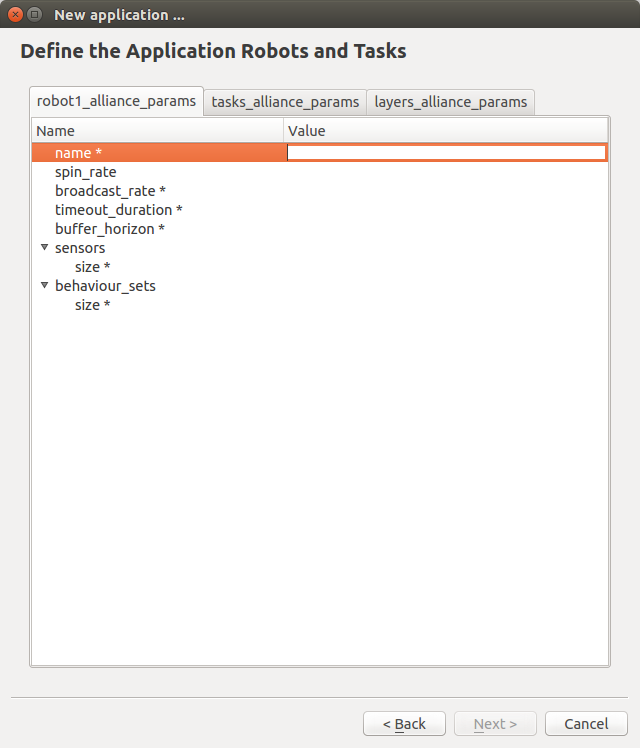
\includegraphics[width=.31\textwidth]{Figuras/3_desenvolvimento/example_def_params.png}
                \label{fig:example_def_params}
            }
            \subfloat[Sumário.]{
                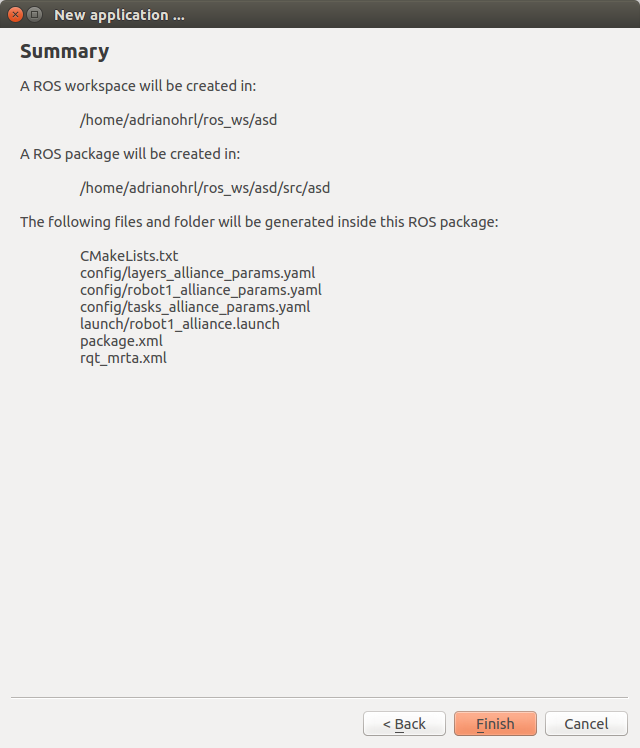
\includegraphics[width=.31\textwidth]{Figuras/3_desenvolvimento/example_summary.png}
                \label{fig:example_summary}
            }
            \caption{\textit{Wizard} para a criação de uma nova aplicação.} \label{fig:example_new_app}
        \end{figure}
        
        A primeira tela do \textit{wizard} de novas aplicações, mostrado na Figura \ref{fig:example_def_app}, coleta os dados gerais da aplicação. Estes dados serão utilizados na geração do arquivo manifesto do pacote. Caso o \textit{workspace} dado não seja um \textit{workspace} do ROS, o usuário é alertado de que será criado um novo \textit{workspace} no diretório especificado. Após o preenchimento de todos os dados obrigatórios, o usuário pode prosseguir para a próxima tela.
        
        Em seguida, pede-se para o usuário escolher uma arquitetura, conforme Figura \ref{fig:example_def_arch}. A escolha pode ser realizada com o auxílio de três filtros: pelo tipo dos robôs (ST \textit{versus} MT), pelo tipo das tarefas (SR \textit{versus} MR) e pelo tipo das alocações (IA \textit{versus} TA), conforme a taxonomia revisada na Seção \ref{subsec:taxonomia_mrta}. Assim que o usuário passa para a próxima tela, o \textit{rqt\_mrta} carrega o arquivo de configuração da arquitetura selecionada. Logo, os \textit{templates} dos arquivos de parâmetro e de inicialização estarão disponíveis na memória.
        
        Após a seleção da arquitetura, pede-se para identificar os robôs do sistema. A interface para a entrada desses dados é mostrada na Figura \ref{fig:example_def_robots}. A partir dos robôs e dos \textit{templates} de arquivos de parâmetro
        
        arquivo de configuração de arquitetura carregado, pede-se para o usuário preencher os arquivos de parâmetros para cada robô, conforme os \textit{templates}, conforme mostra a Figura \ref{fig:example_def_params}.
        
        Os campos que aparecem o símbolo asterisco (*), identificam para o usuário quais entradas devem ser preenchidas obrigatoriamente. O usuário fica impossibilitado de avançar para a próxima tela enquanto ele não tenha preenchido todas entradas obrigatórias. Isso garante que ao final do procedimento, a arquitetura estará devidamente configurada e será possível gerar o pacote da aplicação com sucesso.
        
        \begin{figure}[htb]
            \centering
            \subfloat[Pacote.]{
                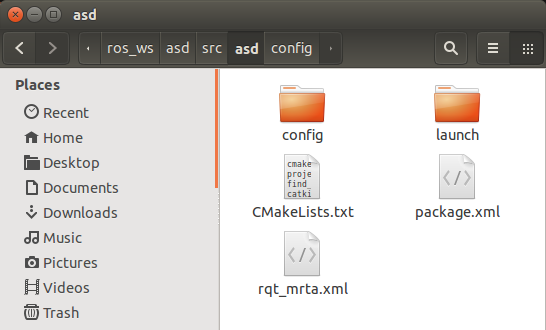
\includegraphics[width=.4\textwidth]{Figuras/3_desenvolvimento/example_pkg.png}
                \label{fig:example_pkg}
            }
            \subfloat[Arquivos de parâmetro.]{
                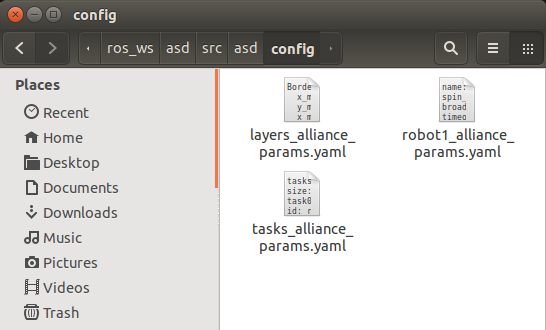
\includegraphics[width=.4\textwidth]{Figuras/3_desenvolvimento/example_pkg_config.png}
                \label{fig:example_pkg_config}
            }
            
            \subfloat[Arquivos de inicialização.]{
                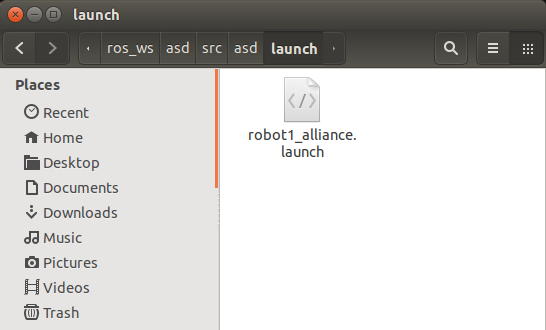
\includegraphics[width=.4\textwidth]{Figuras/3_desenvolvimento/example_pkg_launch.png}
                \label{fig:example_pkg_launch}
            }
            \caption{Pastas e arquivos gerados após a criação de uma aplicação.} \label{fig:example}
        \end{figure}
        
        As Figuras \ref{fig:opening_arch} e \ref{fig:opening_app} mostram, respectivamente, as janelas para a seleção de uma arquitetura e de uma aplicação para o carregamento do seu arquivo de configuração. Ao invés dos usuários navegarem pelos diretórios do sistema operacional procurando o arquivo desejado, são listados para ele os pacotes que foram devidamente configurados, conforme descrito nas Seções \ref{subsec:arch_config} e \ref{subsec:app_config}.
        
        \begin{figure}[htb]
            \centering
            \subfloat[de uma arquitetura.]{
                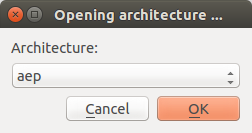
\includegraphics[height=.1\textheight]{Figuras/3_desenvolvimento/opening_arch.png}
                \label{fig:opening_arch}
            }
            \subfloat[de uma aplicação.]{
                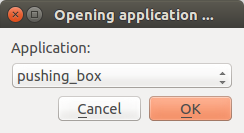
\includegraphics[height=.1\textheight]{Figuras/3_desenvolvimento/opening_app.png}
                \label{fig:opening_app}
            }
            \caption{Carregando um arquivo de configuração} \label{fig:opening_config}
        \end{figure}
        
    \section{Camada de controle} \label{subset:rqt_mrta_controller}
        É mostrado na Figura \ref{fig:rqt_mrta_controller_uml} o diagrama UML (\textit{Unified Modeling Language}) que relaciona as classes do modelo utilizado na camada de modelagem do \textit{rqt\_mrta}. A seguir, serão detalhadas cada classe contida neste diagrama.
        
        \begin{figure}[p]
            \centering
            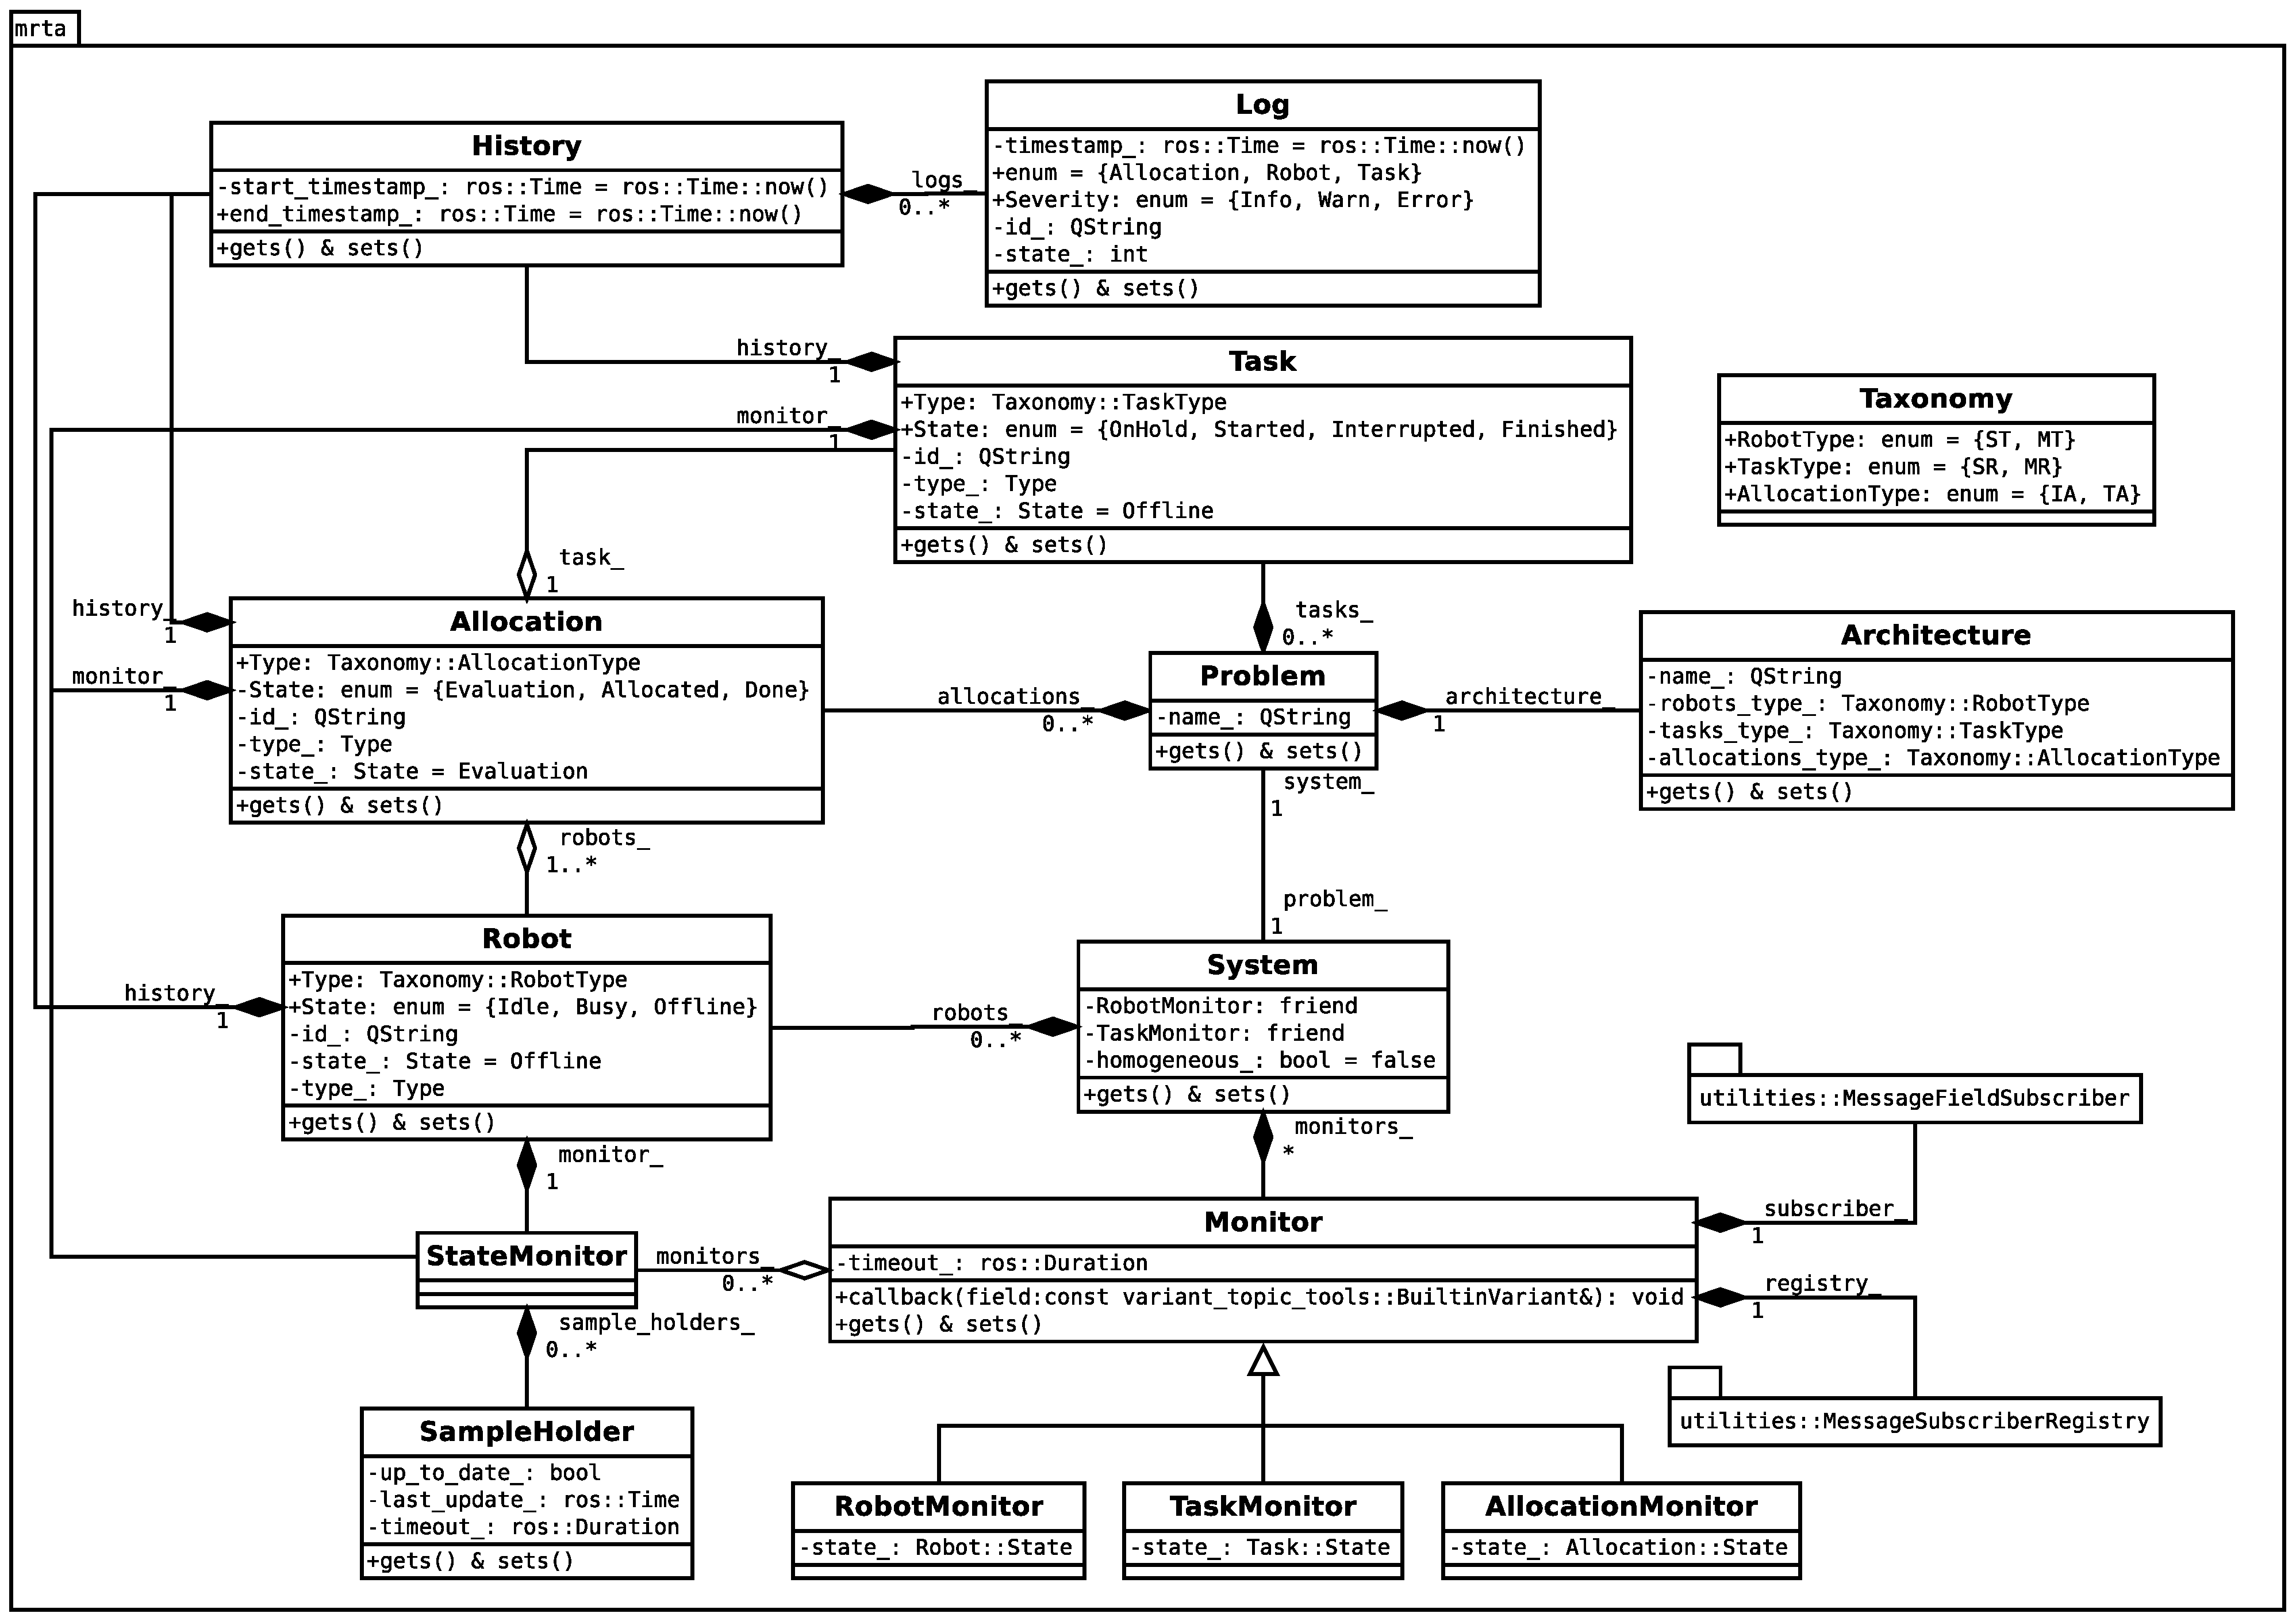
\includegraphics[height=\textwidth,angle=90]{Figuras/3_desenvolvimento/rqt_mrta_controller_uml.eps}
            \caption{Diagrama de classes do camada de controle.} \label{fig:rqt_mrta_controller_uml}
        \end{figure}
        
        A relação entre as classes \textit{System}, \textit{Problem}, \textit{Robot}, \textit{Task}, \textit{Allocation} e \textit{Architecture} se baseia na definição do problema MRTA. Como o sistema possui vários robôs e um problema de alocação de tarefa para ser resolvido, um objeto do tipo \textit{System} é composto por vários objetos do tipo \textit{Robot} e também de uma instância de objeto da classe \textit{Problem}. A classe \textit{Problem} tem como responsabilidade relacionar cada tarefa a ser executada com um robô (caso o tipo das tarefas do sistema seja SR) ou um grupo de robôs (caso o tipo das tarefas do sistema sejam MR) através de uma alocação. Logo, um objeto do tipo \textit{Problem} é composto por vários objetos do tipo \textit{Task}, vários do tipo \textit{Allocation} e uma instância de \textit{Architecture}. A classe \textit{Architecture} apenas armazena a classe de problema que pode ser resolvido pela arquitetura MRTA escolhida. 
        
        As classes \textit{Robot}, \textit{Task} e \textit{Allocation} são muito parecidas. Elas mantêm uma identificação única para cada robô, tarefa e alocação identificados no sistema, respectivamente. Contudo, objetos da classe \textit{Allocation} têm uma instância de \textit{Task} e pode ter um ou vários objetos \textit{Robot}, dependendo do tipo das tarefas que a arquitetura MRTA escolhida resolve. Cada uma dessas três classes ainda possuem um objeto do tipo \textit{History} que armazena \textit{logs} das alterações de estado, o qual é monitorado pelo objeto \textit{StateMonitor} que elas possuem. Objetos \textit{StateMonitor}, por sua vez, são compostos por vários objetos \textit{SampleHolder}, um para cada estado sendo monitorado. Esta classe funciona como se fosse um demultiplexador, direcionando o evento na sua entrada para a saída apropriada. Isto é, se o objeto \textit{StateMonitor} de um dado robô recebe a informação que ele se encontra no estado \textit{Busy} (ocupado), esse encaminha esta informação para o objeto \textit{SampleHolder} que mantém o histórico de notificações desse estado. Portanto, a classe \textit{SampleHolder} é responsável por identificar as rampas de subida e de descida de um dado estado do objeto em monitoramento. Este objeto leva em consideração um parâmetro (\textit{timeout}) que especifica o tempo máximo considerado para manter o dado estado em nível lógico alto.
        
        Voltando a classe \textit{System}, objetos desse tipo ainda são compostos por vários objetos do tipo \textit{Monitor} que pode ser especificado para os tipos \textit{RobotMonitor}, \textit{TaskMonitor} e \textit{AllocationMonitor}. Cada um tem a função de monitorar um campo específico de uma dada mensagem provida de um tópico específico, conforme os parâmetros do arquivo de configuração da arquitetura MRTA escolhida.  Como objeto \textit{Monitor} analisa um estado específico de um conjunto de entidades da mesma natureza. Por exemplo, objetos \textit{RobotMonitor} analisam um dado estado dos robôs do sistema; objetos do tipo \textit{TaskMonitor} analisam um estado específico para as tarefas do sistema; e, por fim, um estado específico das alocações do sistema é analisado em objetos do tipo \textit{AllocationMonitor}. Assim, de forma semelhante à classe \textit{StateMonitor}, as classes do tipo \textit{Monitor} têm um papel similar a um demultiplexador, entregando a notificação recebida ao objeto \textit{StateMonitor} apropriado. Exemplificando, seja um objeto \textit{RobotMonitor} que observa o tópico \textit{/busy\_robots} onde os robôs do sistema publicam quais atividades eles estão desempenhando. Ao ser notificado da chegada de uma mensagem cujo o remetente é o robô \textit{robot1}, este monitor encaminhará uma notificação para o objeto \textit{StateMonitor} do \textit{robot1} dizendo que ele se encontra no estado \textit{Busy}. Por sua vez, o objeto \textit{StateMonitor} de \textit{robot1} direciona está notificação para o \textit{SampleHolder} que mantém o histórico do estado \textit{Busy} de \textit{robot1}. Finalmente, a cada rampa de subida ou descida de um dos seus estados, \textit{robot1} atualiza seu estado atual.
    